\section{Artificial Intelligence\\{\small Paradigmi}} % (fold)
\label{sec:ai_paradigms}
%
\begin{frame}[t,fragile] \frametitle{Intelligenza Artificiale}
{\scriptsize
	\onslide<1->
		\framesubtitle{Secondo il creatore della AI}
		\vspace*{3pt}
		\begin{minipage}[t]{\textwidth}
			\begin{minipage}[t]{0.45\textwidth}
				\centering
				\begin{figure}[ht]
					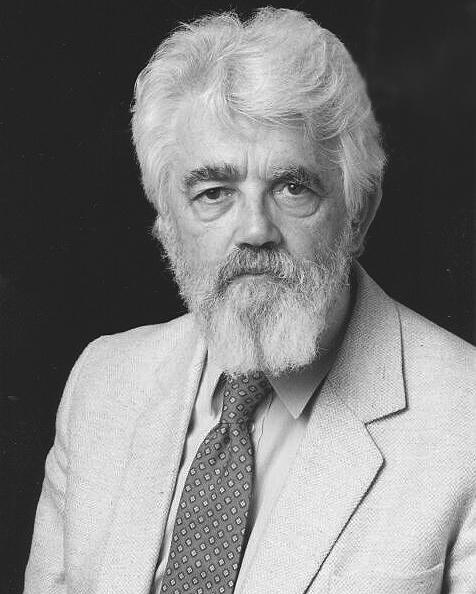
\includegraphics[width=.73\textwidth]{John-McCarthy.jpg}
					{\tiny\\John McCarthy\\\vspace*{-1pt}\textit{\textcopyright Naukas}}
				\end{figure}
			\end{minipage}
		    \begin{minipage}[t]{0.5\textwidth}
				\renewcommand{\epigraphsize}{\small}
				\setlength{\afterepigraphskip}{0pt}
				\setlength{\beforeepigraphskip}{5pt}
				\setlength{\epigraphwidth}{\textwidth}
				\epigraph{
					\textit{\alert{D:} Cosa è l'Intelligenza Artificiale?\\
					\alert{R:} E' la scienza e l'ingegneria di creare macchine intelligenti, in particolare programmi informatici intelligenti. È correlata al compito simile di utilizzare i computer per comprendere l'intelligenza umana, ma l'intelligenza artificiale non deve limitarsi a metodi che siano osservabili biologicamente.}}{John McCarthy, \textbf{Stanford Uni, 2007}\\Traduzione: \textit{\textcopyright ChatGPT}}
			\end{minipage}
		\end{minipage}
}
	\onslide<2->
	\begin{itemize}[leftmargin=10pt,align=right]
		\item[\alert{\faHandORight}] Sistema di AI è un termine estremamente inflazionato\ldots 
		\onslide<3->\item[\alert{\faHandORight}] \ldots anche per sistemi che AI non sono affatto
	\end{itemize}
\end{frame}
%
\begin{frame}[t,fragile] \frametitle{NON Intelligenza Artificiale}
	\vspace*{-15pt}
	\begin{center}
		\begin{minipage}[t]{0.6\textwidth}
			\centering
			\begin{figure}[ht]
				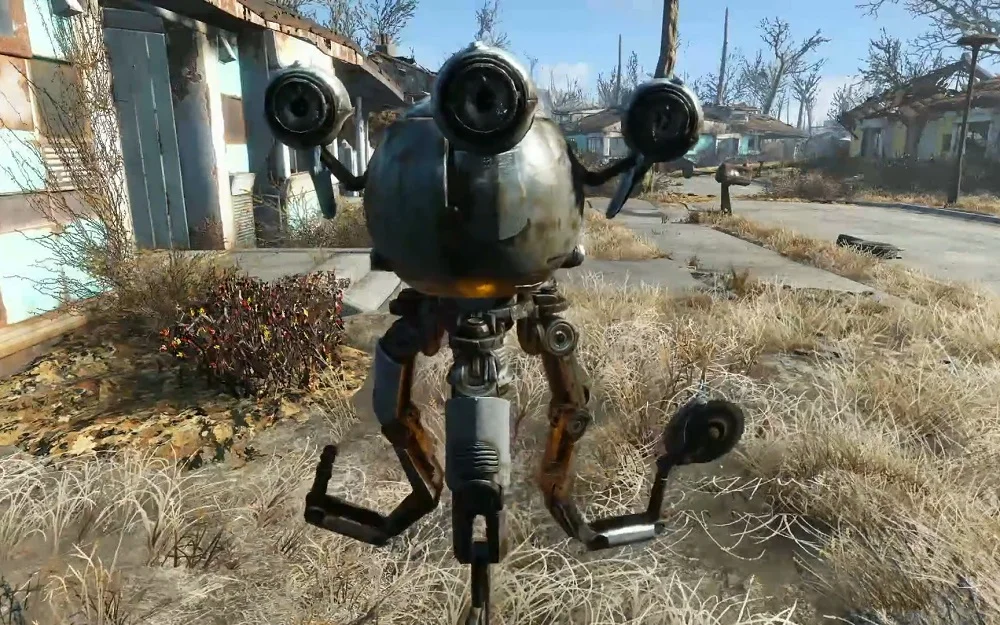
\includegraphics[width=\textwidth]{codsworth.png}
			\end{figure}
		\end{minipage}
		\begin{minipage}[t]{.6\textwidth}
			\renewcommand{\epigraphsize}{\tiny}
			\setlength{\afterepigraphskip}{0pt}
			\setlength{\beforeepigraphskip}{5pt}
			\setlength{\epigraphwidth}{\textwidth}
			\epigraph{\textit{Questo significa che sei, ehm\ldots in ritardo di due secoli per cena! Forse potrei prepararti uno spuntino? Devi essere affamato!}}{Codsworth all'Unico Sopravissuto, \textbf{Fallout 4, 2015}\\\vspace*{0pt}\textit{\textcopyright Nukapedia: The Fallout Wiki}}
		\end{minipage}
	\end{center}
	\onslide<2->
	\begin{itemize}[leftmargin=10pt,align=right]
		\item[\alert{\faHandORight}] \alert{\textit{Non-Playable Characters}} (NPC) dei \textit{videogame} 
		\onslide<3->\item[\alert{\faHandORight}] Sistemi di regole \textit{if-then-else}, \alert{non} AI
	\end{itemize}
\end{frame}
%
\section{AI: Debole vs Forte} % (fold)
\label{sec:ai_types}
%
\begin{frame}[t,fragile] \frametitle{Artificial Intelligence}
	{\footnotesize
		\onslide<1->
            \framesubtitle{Due paradigmi a confronto}
            \vspace*{-15pt}
            \begin{minipage}[t]{\textwidth}
             	%\begin{figure}[ht]
                %    \centering
                %    \includegraphics[width=\textwidth]{AI-paradigms-timeline.png}
                %\end{figure}
            \end{minipage}
            \\\vspace*{3pt}
	    	\begin{minipage}[t]{\textwidth}
				\begin{minipage}[t]{0.6\textwidth}
	    			\begin{itemize}[leftmargin=10pt,align=right]
						\onslide<2->\item[\alert{\faHandORight}] \alert{AI Debole (Narrow AI):} sistemi specializzati per compiti specifici
						\onslide<3->\item[\alert{\faHandORight}] \alert{AI Forte (General AI):} sistemi con intelligenza simile a quella umana
						\onslide<4->\item[\alert{\faHandORight}] \alert{Super AI:} intelligenza che supera quella umana in tutti i domini
						\onslide<5->\item[\alert{\faHandORight}] Oggi esistono \alert{solo} sistemi di AI Debole
					\end{itemize}
            	\end{minipage}
            	%
				\onslide<1->
            	\begin{minipage}[t]{0.4\textwidth}
                	\centering
                	%\begin{figure}[ht]
                    %	\includegraphics[width=.8\textwidth]{ai-evolution.png}
                    %	{\tiny\\Evoluzione dell'AI\\\vspace*{-1pt}\textit{\textcopyright AI Research}}
                	%\end{figure}
            	\end{minipage}
	    	\end{minipage}
	}
\end{frame}
%
\begin{frame}[t,fragile] \frametitle{AI Debole (Narrow AI)}
	{\scriptsize
		\onslide<1->
            \framesubtitle{Specializzazione in domini ristretti}
            \vspace*{-10pt}
	    	\begin{minipage}[t]{\textwidth}
				\begin{minipage}[t]{0.6\textwidth}
	    			\begin{itemize}[leftmargin=10pt,align=right]
						\onslide<2->\item[\alert{\faHandORight}] \alert{Definizione:} sistemi progettati per eccellere in \alert{un singolo compito specifico}
						\onslide<3->\item[\alert{\faHandORight}] \alert{Caratteristiche:}
						\begin{itemize}[leftmargin=10pt,align=right]
							\item[\alert{\faHandORight}] Dominio limitato e ben definito
							\item[\alert{\faHandORight}] Performance superiori all'umano nel loro campo
							\item[\alert{\faHandORight}] Incapaci di generalizzare oltre il loro scopo
						\end{itemize}
						\onslide<4->\item[\alert{\faHandORight}] \alert{Esempi quotidiani:}
						\begin{itemize}[leftmargin=10pt,align=right]
							\item[\alert{\faHandORight}] Riconoscimento vocale (Siri, Alexa)
							\item[\alert{\faHandORight}] Raccomandazioni (Netflix, Spotify)
							\item[\alert{\faHandORight}] Traduzione automatica (Google Translate)
						\end{itemize}
					\end{itemize}
            	\end{minipage}
            	%
				\onslide<1->
            	\begin{minipage}[t]{0.4\textwidth}
                	\centering
                	%\begin{figure}[ht]
                    %	\includegraphics[width=.8\textwidth]{narrow-ai-examples.png}
                    %	{\tiny\\AI Debole: esempi\\\vspace*{-1pt}\textit{\textcopyright Tech Illustrations}}
                	%\end{figure}
            	\end{minipage}
	    	\end{minipage}
	}
\end{frame}
%
\begin{frame}[t,fragile] \frametitle{AI Debole: Esempi per Sviluppatori}
	{\small
		\onslide<1->
		\framesubtitle{Casi d'uso in ambito Spring Boot}
		\begin{itemize}[leftmargin=10pt,align=right]
			\onslide<2->\item[\alert{\faHandORight}] \alert{Analisi del sentiment:} classificare recensioni dei clienti
			\onslide<3->\item[\alert{\faHandORight}] \alert{Chatbot per supporto:} rispondere a domande frequenti
			\onslide<4->\item[\alert{\faHandORight}] \alert{Rilevamento frodi:} identificare transazioni sospette
			\onslide<5->\item[\alert{\faHandORight}] \alert{Ottimizzazione prezzi:} adeguare prezzi in base alla domanda
		\end{itemize}
		\vspace*{.3cm}
		\only<2|handout:1>{
		\begin{minipage}[t]{\textwidth}
			\begin{minipage}[t]{0.6\textwidth}
				\renewcommand{\epigraphsize}{\scriptsize}
				\setlength{\afterepigraphskip}{0pt}
				\setlength{\beforeepigraphskip}{5pt}
				\setlength{\epigraphwidth}{0.9\textwidth}
				\epigraph{\textit{@RestController\\
public class SentimentController \{\\
\quad @Autowired\\
\quad private SentimentAnalysisService service;\\
\quad\\
\quad @PostMapping("/analyze")\\
\quad public SentimentResult analyze(@RequestBody String text) \{\\
\quad\quad return service.analyzeSentiment(text);\\
\quad \}\\
\}}}{Esempio Spring Boot per analisi sentiment}
			\end{minipage}
			\begin{minipage}[t]{0.35\textwidth}
				\centering
				%\begin{figure}[ht]
				%	\includegraphics[width=.8\textwidth]{sentiment-analysis.png}
				%	{\tiny\\Analisi del Sentiment\\\vspace*{-4pt}\textit{\textcopyright ML Concepts}}
				%\end{figure}
			\end{minipage}
		\end{minipage}
		}
		\only<3|handout:2>{
		\begin{minipage}[t]{\textwidth}
			\begin{minipage}[t]{0.6\textwidth}
				\renewcommand{\epigraphsize}{\scriptsize}
				\setlength{\afterepigraphskip}{0pt}
				\setlength{\beforeepigraphskip}{5pt}
				\setlength{\epigraphwidth}{0.9\textwidth}
				\epigraph{\textit{@Component\\
public class ChatbotService \{\\
\quad\\
\quad public String processQuery(String userQuery) \{\\
\quad\quad if (userQuery.contains("password")) \{\\
\quad\quad\quad return "Per resettare la password...";\\
\quad\quad \}\\
\quad\quad // Pattern matching limitato\\
\quad\quad return "Non ho capito la domanda";\\
\quad \}\\
\}}}{Chatbot tradizionale (regole fisse)}
			\end{minipage}
			\begin{minipage}[t]{0.35\textwidth}
				\centering
				%\begin{figure}[ht]
				%	\includegraphics[width=.8\textwidth]{chatbot-rules.png}
				%	{\tiny\\Chatbot a regole\\\vspace*{-4pt}\textit{\textcopyright Bot Design}}
				%\end{figure}
			\end{minipage}
		\end{minipage}
		}
		\only<4|handout:3>{
		\begin{minipage}[t]{\textwidth}
			\begin{minipage}[t]{0.6\textwidth}
				\renewcommand{\epigraphsize}{\scriptsize}
				\setlength{\afterepigraphskip}{0pt}
				\setlength{\beforeepigraphskip}{5pt}
				\setlength{\epigraphwidth}{0.9\textwidth}
				\epigraph{\textit{@Service\\
public class FraudDetectionService \{\\
\quad\\
\quad public boolean isFraudulent(Transaction tx) \{\\
\quad\quad // Analizza pattern: importo, orario, \\
\quad\quad // geolocalizzazione, frequenza\\
\quad\quad return mlModel.predict(tx.getFeatures()) > 0.8;\\
\quad \}\\
\}}}{Sistema di rilevamento frodi basato su ML}
			\end{minipage}
			\begin{minipage}[t]{0.35\textwidth}
				\centering
				%\begin{figure}[ht]
				%	\includegraphics[width=.8\textwidth]{fraud-detection.png}
				%	{\tiny\\Rilevamento Frodi\\\vspace*{-4pt}\textit{\textcopyright FinTech AI}}
				%\end{figure}
			\end{minipage}
		\end{minipage}
		}
		\only<5|handout:4>{
		\begin{minipage}[t]{\textwidth}
			\begin{minipage}[t]{0.6\textwidth}
				\renewcommand{\epigraphsize}{\scriptsize}
				\setlength{\afterepigraphskip}{0pt}
				\setlength{\beforeepigraphskip}{5pt}
				\setlength{\epigraphwidth}{0.9\textwidth}
				\epigraph{\textit{@RestController\\
public class PricingController \{\\
\quad @Autowired\\
\quad private DynamicPricingService pricingService;\\
\quad\\
\quad @GetMapping("/price/\{productId\}")\\
\quad public PriceResponse getPrice(@PathVariable Long productId,\\
\quad\quad\quad\quad\quad\quad\quad\quad\quad\quad @RequestParam String customerSegment) \{\\
\quad\quad return pricingService.calculateOptimalPrice(productId, customerSegment);\\
\quad \}\\
\}}}{Pricing dinamico basato su AI}
			\end{minipage}
			\begin{minipage}[t]{0.35\textwidth}
				\centering
				%\begin{figure}[ht]
				%	\includegraphics[width=.8\textwidth]{dynamic-pricing.png}
				%	{\tiny\\Pricing Dinamico\\\vspace*{-4pt}\textit{\textcopyright E-commerce AI}}
				%\end{figure}
			\end{minipage}
		\end{minipage}
		}
	}
\end{frame}
%
\begin{frame}[t,fragile] \frametitle{AI Forte (Artificial General Intelligence)}
	{\scriptsize
		\onslide<1->
            \framesubtitle{Il sogno dell'intelligenza universale}
            \vspace*{-10pt}
	    	\begin{minipage}[t]{\textwidth}
				\begin{minipage}[t]{0.6\textwidth}
	    			\begin{itemize}[leftmargin=10pt,align=right]
						\onslide<2->\item[\alert{\faHandORight}] \alert{Definizione:} sistemi con \alert{intelligenza generale} comparabile a quella umana
						\onslide<3->\item[\alert{\faHandORight}] \alert{Caratteristiche teoriche:}
						\begin{itemize}[leftmargin=10pt,align=right]
							\item[\alert{\faHandORight}] Capacità di ragionamento astratto
							\item[\alert{\faHandORight}] Apprendimento da esperienze limitate
							\item[\alert{\faHandORight}] Trasferimento di conoscenza tra domini
							\item[\alert{\faHandORight}] Creatività e intuizione
						\end{itemize}
						\onslide<4->\item[\alert{\faHandORight}] \alert{Status attuale:} \alert{NON ESISTE}
						\onslide<5->\item[\alert{\faHandORight}] \alert{Stime degli esperti:} 2045-2100 (molto incerto)
					\end{itemize}
            	\end{minipage}
            	%
				\onslide<1->
            	\begin{minipage}[t]{0.4\textwidth}
                	\centering
                	%\begin{figure}[ht]
                    % 	\includegraphics[width=.8\textwidth]{agi-concept.png}
                    %	{\tiny\\Concetto di AGI\\\vspace*{-1pt}\textit{\textcopyright Future AI}}
                	%\end{figure}
            	\end{minipage}
	    	\end{minipage}
	}
\end{frame}
%
\begin{frame}[t,fragile] \frametitle{AI Forte: Esempi Ipotetici}
	{\small
		\onslide<1->
		\framesubtitle{Cosa potrebbe fare un'AGI}
		\begin{itemize}[leftmargin=10pt,align=right]
			\onslide<2->\item[\alert{\faHandORight}] \alert{Programmatore universale:} scrivere codice in qualsiasi linguaggio e dominio
			\onslide<3->\item[\alert{\faHandORight}] \alert{Problem solver generale:} risolvere problemi mai visti prima
			\onslide<4->\item[\alert{\faHandORight}] \alert{Apprendimento rapido:} imparare nuovi concetti da pochi esempi
			\onslide<5->\item[\alert{\faHandORight}] \alert{Ragionamento causale:} comprendere cause ed effetti complessi
		\end{itemize}
		\vspace*{.3cm}
		\only<2|handout:1>{
		\begin{minipage}[t]{\textwidth}
			\begin{minipage}[t]{0.6\textwidth}
				\renewcommand{\epigraphsize}{\scriptsize}
				\setlength{\afterepigraphskip}{0pt}
				\setlength{\beforeepigraphskip}{5pt}
				\setlength{\epigraphwidth}{0.9\textwidth}
				\epigraph{\textit{AGI: "Analizzerò il tuo sistema legacy in COBOL, lo convertirò in microservizi Spring Boot, ottimizzerò le performance del database, implementerò la sicurezza OAuth2 e creerò una UI React responsive. Tutto completato in 30 minuti."}}{Scenario ipotetico di AGI programmatore}
			\end{minipage}
			\begin{minipage}[t]{0.35\textwidth}
				\centering
				%\begin{figure}[ht]
				%	\includegraphics[width=.8\textwidth]{universal-programmer.png}
				%	{\tiny\\Programmatore Universale\\\vspace*{-4pt}\textit{\textcopyright Sci-Fi Tech}}
				%\end{figure}
			\end{minipage}
		\end{minipage}
		}
		\only<3|handout:2>{
		\begin{minipage}[t]{\textwidth}
			\begin{minipage}[t]{0.6\textwidth}
				\renewcommand{\epigraphsize}{\scriptsize}
				\setlength{\afterepigraphskip}{0pt}
				\setlength{\beforeepigraphskip}{5pt}
				\setlength{\epigraphwidth}{0.9\textwidth}
				\epigraph{\textit{AGI: "Il tuo e-commerce ha un calo delle vendite del 23\%. Dopo aver analizzato dati di mercato, comportamento utenti e tendenze sociali, ho identificato 12 fattori causali e propongo una strategia integrata che combina UX, pricing e marketing personalizzato."}}{Scenario di problem solving generale}
			\end{minipage}
			\begin{minipage}[t]{0.35\textwidth}
				\centering
				%\begin{figure}[ht]
				%	\includegraphics[width=.8\textwidth]{general-problem-solver.png}
				%	{\tiny\\Problem Solver Generale\\\vspace*{-4pt}\textit{\textcopyright AI Concepts}}
				%\end{figure}
			\end{minipage}
		\end{minipage}
		}
		\only<4|handout:3>{
		\begin{minipage}[t]{\textwidth}
			\begin{minipage}[t]{0.6\textwidth}
				\renewcommand{\epigraphsize}{\scriptsize}
				\setlength{\afterepigraphskip}{0pt}
				\setlength{\beforeepigraphskip}{5pt}
				\setlength{\epigraphwidth}{0.9\textwidth}
				\epigraph{\textit{AGI: "Non ho mai visto il framework Quantum-Spring che avete appena rilasciato, ma dopo aver letto 3 esempi di codice ho compreso i pattern architetturali e posso già ottimizzare la vostra implementazione."}}{Apprendimento rapido da pochi esempi}
			\end{minipage}
			\begin{minipage}[t]{0.35\textwidth}
				\centering
				%\begin{figure}[ht]
				%	\includegraphics[width=.8\textwidth]{rapid-learning.png}
				%	{\tiny\\Apprendimento Rapido\\\vspace*{-4pt}\textit{\textcopyright Learning AI}}
				%\end{figure}
			\end{minipage}
		\end{minipage}
		}
		\only<5|handout:4>{
		\begin{minipage}[t]{\textwidth}
			\begin{minipage}[t]{0.6\textwidth}
				\renewcommand{\epigraphsize}{\scriptsize}
				\setlength{\afterepigraphskip}{0pt}
				\setlength{\beforeepigraphskip}{5pt}
				\setlength{\epigraphwidth}{0.9\textwidth}
				\epigraph{\textit{AGI: "Il bug nel vostro sistema non è dove pensate. Il vero problema è un race condition causato da un pattern di design che crea dipendenze cicliche tra tre microservizi, amplificato dal garbage collector di JVM sotto carico elevato."}}{Ragionamento causale profondo}
			\end{minipage}
			\begin{minipage}[t]{0.35\textwidth}
				\centering
				%\begin{figure}[ht]
				%	\includegraphics[width=.8\textwidth]{causal-reasoning.png}
				%	{\tiny\\Ragionamento Causale\\\vspace*{-4pt}\textit{\textcopyright Logic AI}}
				%\end{figure}
			\end{minipage}
		\end{minipage}
		}
	}
\end{frame}
%
\begin{frame}[t,fragile] \frametitle{Confronto: AI Debole vs AI Forte}
	{\small
		\framesubtitle{Differenze pratiche per lo sviluppatore}
		\vspace*{-.5cm}
		\begin{center}
		{\scriptsize
		\begin{table}
			\setlength{\tabcolsep}{8pt}
			\renewcommand{\arraystretch}{1.5}
			\centering
			\begin{tabular}{p{2.5cm}p{4cm}p{4cm}}
				\toprule
				\textbf{Aspetto} & \textbf{AI Debole (Narrow)} & \textbf{AI Forte (General)}\\
				\midrule
				\alert{Scopo} & Un singolo compito specifico & Qualsiasi compito cognitivo\\
				\alert{Apprendimento} & Dataset grandi, training lungo & Pochi esempi, apprendimento rapido\\
				\alert{Trasferibilità} & Zero (limitata al dominio) & Totale (tra qualsiasi dominio)\\
				\alert{Creatività} & Assente o molto limitata & Creatività genuina\\
				\alert{Ragionamento} & Pattern matching avanzato & Comprensione causale\\
				\alert{Implementazione} & Disponibile oggi & Non esiste ancora\\
				\alert{Costo/Complessità} & Gestibile per singoli casi d'uso & Teoricamente enorme\\
				\alert{Esempio Spring} & Servizio di sentiment analysis & "Assistente" che scrive, debugga, ottimizza e mantiene tutto il codice\\
				\bottomrule
			\end{tabular}
		\end{table}
		}
		\end{center}
	}
\end{frame}
%
\begin{frame}[t,fragile] \frametitle{Spring AI e AI Debole}
	{\small
		\onslide<1->
		\framesubtitle{Focus pratico per il vostro lavoro}
		\begin{itemize}[leftmargin=10pt,align=right]
			\onslide<2->\item[\alert{\faHandORight}] \alert{Spring AI si concentra su AI Debole:} integrazioni pratiche e immediate
			\onslide<3->\item[\alert{\faHandORight}] \alert{Vantaggi dell'approccio Narrow AI:}
			\begin{itemize}[leftmargin=10pt,align=right]
				\item[\alert{\faHandORight}] Risultati misurabili e predicibili
				\item[\alert{\faHandORight}] ROI chiaro e immediato
				\item[\alert{\faHandORight}] Rischi controllabili
			\end{itemize}
			\onslide<4->\item[\alert{\faHandORight}] \alert{Esempi concreti con Spring AI:}
			\begin{itemize}[leftmargin=10pt,align=right]
				\item[\alert{\faHandORight}] Integrazione con OpenAI, Azure AI, AWS Bedrock
				\item[\alert{\faHandORight}] Vector databases per RAG
				\item[\alert{\faHandORight}] Embedding e similarity search
			\end{itemize}
		\end{itemize}
		\vspace*{.3cm}
		\only<4|handout:1>{
		\begin{minipage}[t]{\textwidth}
			\renewcommand{\epigraphsize}{\scriptsize}
			\setlength{\afterepigraphskip}{0pt}
			\setlength{\beforeepigraphskip}{5pt}
			\setlength{\epigraphwidth}{0.9\textwidth}
			\epigraph{\textit{@RestController\\
public class AIController \{\\
\quad @Autowired\\
\quad private ChatClient chatClient;\\
\quad\\
\quad @PostMapping("/chat")\\
\quad public String chat(@RequestBody String prompt) \{\\
\quad\quad return chatClient.call(prompt);\\
\quad \}\\
\}}}{Spring AI: semplicità nell'integrazione}
		\end{minipage}
		}
	}
\end{frame}
%
\begin{frame}[t,fragile] \frametitle{Takeaway per il Developer}
	{\small
		\framesubtitle{Cosa ricordare}
		\begin{itemize}[leftmargin=10pt,align=right]
			\item[\alert{\faHandORight}] \alert{AI Debole è realtà:} tecnologie mature e utilizzabili oggi
			\item[\alert{\faHandORight}] \alert{AI Forte è futuro:} interessante teoricamente, ma non influenza le decisioni tecniche attuali
			\item[\alert{\faHandORight}] \alert{Focus sul valore immediato:} identificare problemi specifici che l'AI Debole può risolvere
			\item[\alert{\faHandORight}] \alert{Spring AI è il ponte:} semplifica l'integrazione di AI Debole nelle applicazioni enterprise
		\end{itemize}
		\vspace*{.5cm}
		\begin{center}
			\alert{\Large Non aspettare l'AGI: inizia oggi con l'AI Debole!}
		\end{center}
	}
\end{frame}
%